\let\negmedspace\undefined
\let\negthickspace\undefined
\documentclass[journal]{IEEEtran}
\usepackage[a5paper, margin=10mm, onecolumn]{geometry}
%\usepackage{lmodern} % Ensure lmodern is loaded for pdflatex
\usepackage{tfrupee} % Include tfrupee package

\setlength{\headheight}{1cm} % Set the height of the header box
\setlength{\headsep}{0mm}     % Set the distance between the header box and the top of the text

\usepackage{gvv-book}
\usepackage{gvv}
\usepackage{cite}
\usepackage{amsmath,amssymb,amsfonts,amsthm}
\usepackage{algorithmic}
\usepackage{graphicx}
\usepackage{textcomp}
\usepackage{xcolor}
\usepackage{txfonts}
\usepackage{listings}
\usepackage{enumitem}
\usepackage{mathtools}
\usepackage{gensymb}
\usepackage{comment}
\usepackage[breaklinks=true]{hyperref}
\usepackage{tkz-euclide} 
\usepackage{listings}
% \usepackage{gvv}                                        
\def\inputGnumericTable{}                                 
\usepackage[latin1]{inputenc}                                
\usepackage{color}                                            
\usepackage{array}                                            
\usepackage{longtable}                                       
\usepackage{calc}                                             
\usepackage{multirow}                                         
\usepackage{hhline}                                           
\usepackage{ifthen}                                           
\usepackage{lscape}
\begin{document}

\bibliographystyle{IEEEtran}
\vspace{3cm}

\title{2.7.13}
\author{EE25BTECH11001 - Aarush Dilawri}
% \maketitle
% \newpage
% \bigskip
{\let\newpage\relax\maketitle}

\renewcommand{\thefigure}{\theenumi}
\renewcommand{\thetable}{\theenumi}
\setlength{\intextsep}{10pt} % Space between text and floats
\textbf{Question}:\\
Given vertices $\vec{A}(-4,-5)$, $\vec{B}(-1,-6)$ , $\vec{C}(-5,7)$ and $\vec{D}(4,5)$ of a quadrilateral. Find the area of quadrilateral $ABCD$.\\
\textbf{Solution}:\\


Given vertices $\vec{A}=\myvec{-4\\-5}$, $\vec{B}=\myvec{-1\\-6}$, $\vec{C}=\myvec{-5\\7}$, $\vec{D}=\myvec{4\\5}$.  
We split the quadrilateral into triangles $\triangle ABC$ and $\triangle ACD$ and add them to get the answer.




\textbf{Area of $\triangle ABC$:}

\begin{align}
\text{Area}_{ABC}
&= \tfrac{1}{2}\,\big\lVert (\vec{B}-\vec{A}) \times (\vec{C}-\vec{A}) \big\rVert = 17.5
\end{align}

\textbf{Area of $\triangle ACD$:}

\begin{align}
\text{Area}_{ACD}
&= \tfrac{1}{2}\,\big\lVert (\vec{C}-\vec{A}) \times (\vec{D}-\vec{A}) \big\rVert = 53
\end{align}

\textbf{Total area of quadrilateral (sum of triangle areas):}

\begin{align}
\text{Area}_{ABCD} &= \text{Area}_{ABC} + \text{Area}_{ACD} = 70.5
\end{align}
\newpage
See Fig. 0 ,
\begin{figure}[H]
\begin{center}
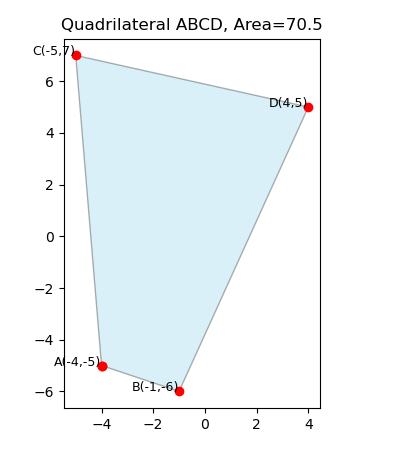
\includegraphics[width=0.6\columnwidth]{figs/fig.png}
\end{center}
\caption{}
\label{fig:Fig1}
\end{figure}
\end{document}
